\documentclass{article}
\usepackage[utf8]{inputenc}
\usepackage{amsmath}
\usepackage{amssymb}
\usepackage{amsfonts}
\usepackage[dvipsnames]{xcolor}
\usepackage{listings}
\usepackage{graphicx}
\usepackage{float}
\usepackage{hyperref} 

\setlength{\parskip}{03pt} % default: \parskip = 12  pt

\newcommand{\bs}[1]{\boldsymbol{#1}}

\title{MAT 167 WQ 2024 Final Programming Project Report}
\author{Alison Wong}
\date{\today}

\setlength{\textheight}{ 620 pt}
\setlength{\voffset}{-20 pt}
\setlength{\headsep}{12 pt}
\setlength{\headheight}{14 pt}
\setlength{\topskip}{12 pt}
\setlength{\footskip}{30 pt}


\usepackage{fancyhdr}
\pagestyle{fancy}
\fancyhead{}

\fancyhead[L]{\textbf{NAME: Alison Wong}}
\fancyhead[C]{\textbf{FPP}}
\fancyhead[R]{\textbf{SID: 918258892}}

\fancyfoot[L]{CRN 30769}
\fancyfoot[C]{--~\thepage~--}
\fancyfoot[R]{\today}

\begin{document}

\maketitle
\tableofcontents
\newpage

\section{Problem Description}

The motivation for this study arises from the practical importance of accurately classifying handwritten digits in various real-world scenarios. For instance, in postal services, automated sorting of mail relies on accurately recognizing handwritten zip codes and addresses. 

Improving the accuracy of handwritten digit classification algorithms can lead to significant advancements such as document processing and data entry automation. Therefore, exploring and comparing different classification approaches is crucial for identifying the most effective methods and optimizing their performance. In this project, we aim to investigate and evaluate two distinct classification algorithms: a centroid classification algorithm and a more sophisticated and accurate approach utilizing singular value decomposition (SVD). Through this comparative analysis, we seek to gain insights into the strengths and limitations of each method by comparing their confusion matrix. The program is performed in MATLAB.

\section{Data Set}

This USPS.mat contains four arrays derived from the U.S. Postal Service database, which can be found \href{https://gaussianprocess.org/gpml/data/}{here}:
\textit{train patterns} and \textit{test patterns} of size ($256 \times 4649$) and
\textit{train labels} and \textit{test labels} of size ($10 \times 4649$).

The arrays \textit{train patterns} and \textit{test patterns} contain a raster scan of the $16 \times 16$ gray level pixel intensities that have been normalized to lie within the range $[-1, 1]$. Each column represents a single train/test image and the elements in each column correspond to the pixel intensities of the image. The digit images in the training set are used to train our algorithm to know which digits they are, in our case, using the mean digit images. The testing data is used to evaluate the accuracy of the trained algorithm. 

The arrays {train labels} and \textit{test labels} contain true information about the digit images.

Figure 1 displays the first 16 images in \textit{train patterns}.
\begin{figure}[H]
\centering
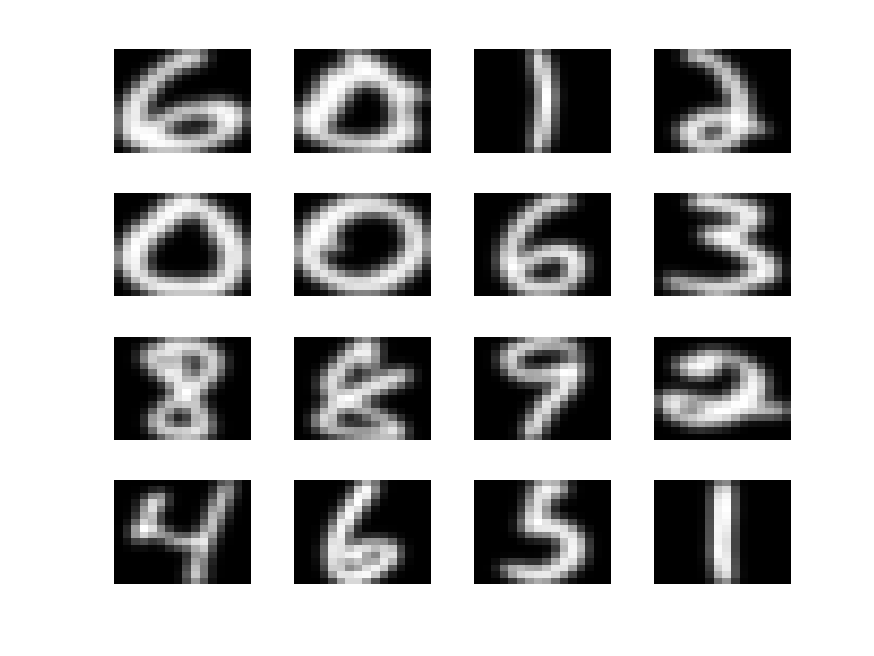
\includegraphics[scale=0.5]{first_16_images.png}
\caption[\abovecaptionskip=18pt]{First 16 Images in Training Set}
\label{FIG:FIG 01}
\end{figure}

We can see that there is variability in handwriting for each digit that our classification algorithm has to take into account. 

\section{The Centroid Classification Algorithm}

The centroid classification algorithm is a simple classification algorithm performed by obtaining the squared Euclidean distances between the testing set and each of the mean digit images from the testing data. 

\subsection{Description of the Algorithm}

Finding the mean digits is crucial for understanding the overall characteristics of each digit class. To calculate the mean digit image for each class, we average the pixel intensities of all images belonging to the same digit class. 

\[
\text{mean\_digit\_image}_k = \frac{1}{n_k} \sum_{i=1}^{n_k} \text{image}_i^{(k)}, \text{k: digit class}
\]

\begin{figure}[H]
\centering
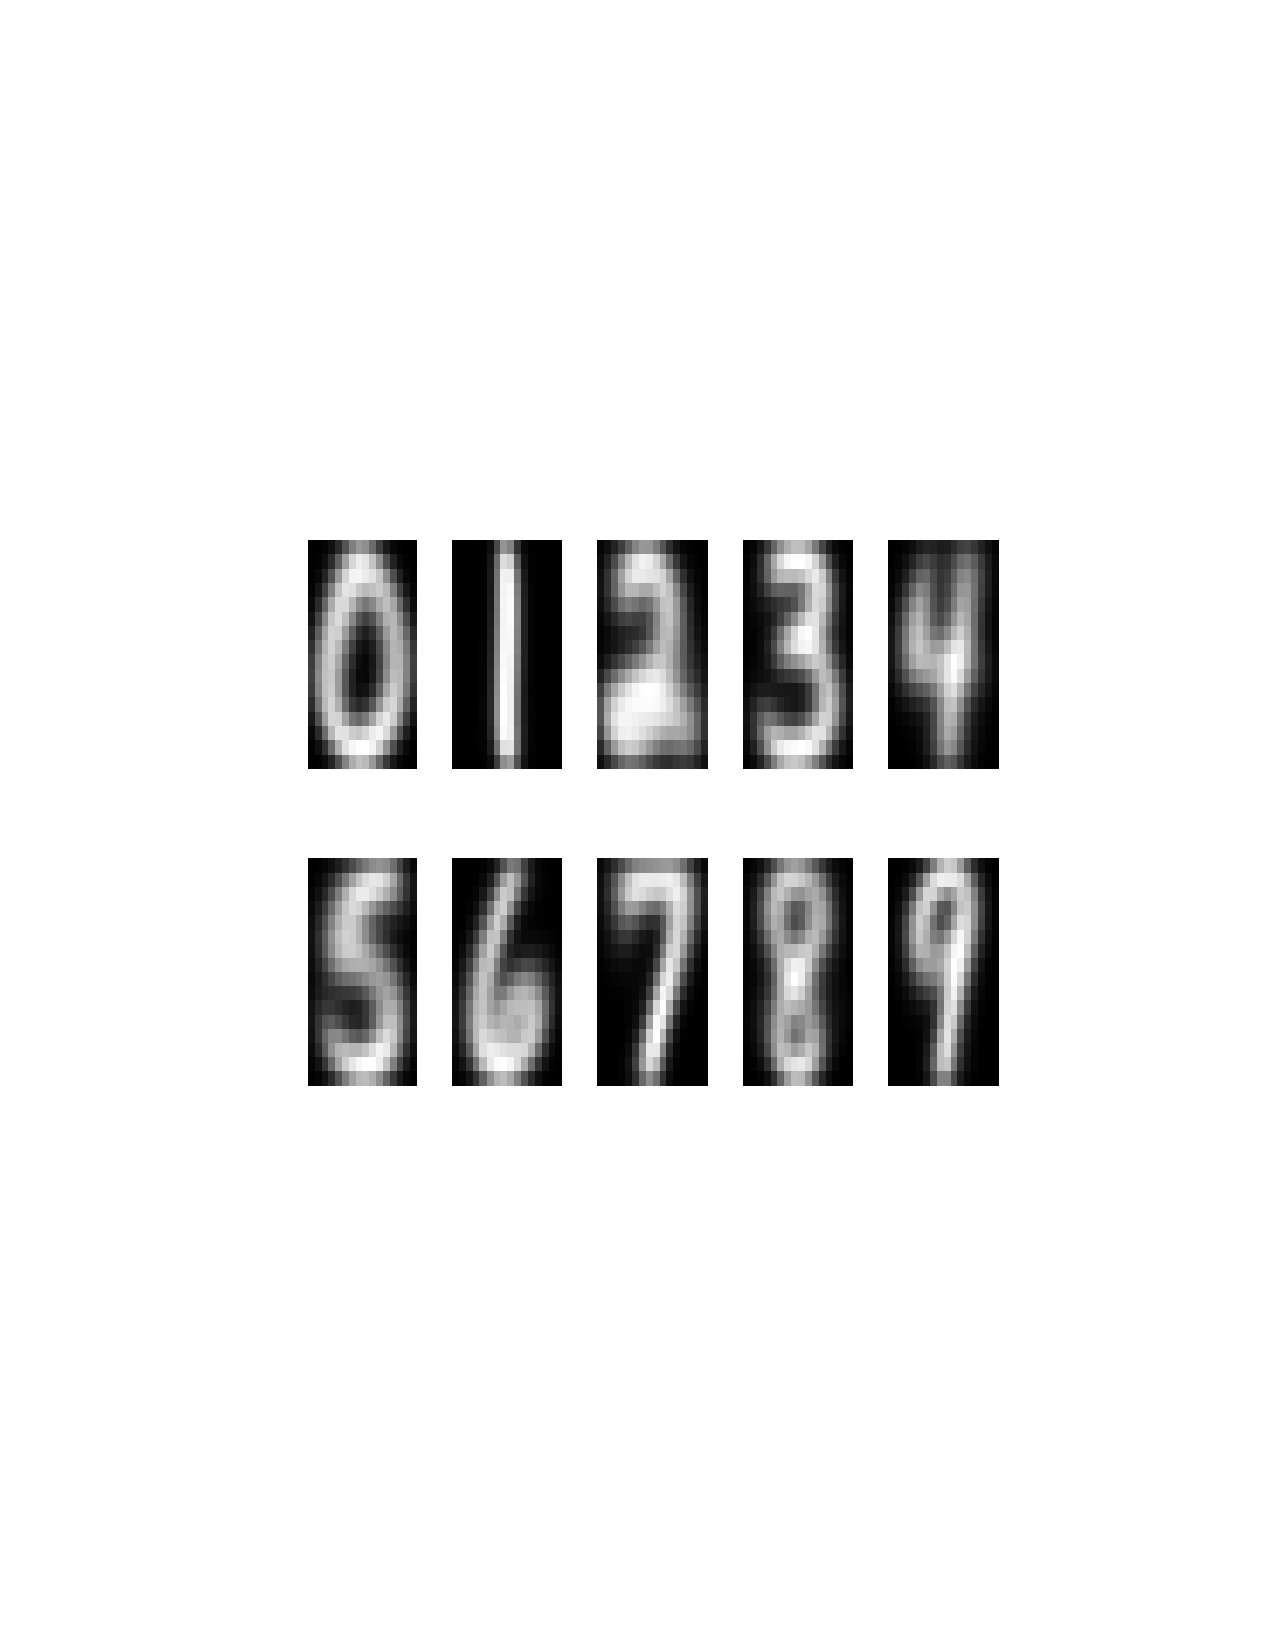
\includegraphics[scale=0.5]{mean_digit_images.pdf}
\caption[\abovecaptionskip=18pt]{The means of all digits in the training set}
\label{FIG:FIG 02}
\end{figure}

In Figure 2, we illustrated the means (centroids) of the digits in the training set. From the figure, we get the impression that a majority of the digits are well-written. 

We obtain a representative image from the mean digit that captures the average pixel intensity values across all training samples belonging to the same digit class. This allows us to visualize the typical appearance of each digit and identify any distinctive features. Analyzing the mean digit images can also provide insights into the variability within each digit class and potential challenges in classification.

After obtaining the squared Euclidean distances between the testing set and each of the mean digit images from the testing data, for each digit in the testing set, the minimum squared Euclidean distance with the mean digit images is classified as that digit class. The classification results indicate how well the algorithm performs in identifying the correct digit class for each test image. 

\[
\text{distance}^2 = \sum_{i=1}^{256} (\text{test\_pattern}_i - \text{mean\_digit\_image}_i)^2
\]

\subsection{Description of the Results}

The confusion matrix provides a detailed breakdown of the classification accuracy for each digit class, showing the number of correctly classified instances and misclassifications by comparing the classification with the \textit{test labels}.

In a confusion matrix:
\begin{itemize}
\item Rows represent the true classes
\item Columns represent the predicted classes
\item Diagonal entries represent the instances that are correctly classified, predicted class = actual class
\item Off-diagonal entries represent misclassifications
\end{itemize}

\[
\begin{bmatrix}
656 & 1 & 3 & 4 & 10 & 19 & 73 & 2 & 17 & 1 \\
0 & 644 & 0 & 1 & 0 & 0 & 1 & 0 & 1 & 0 \\
14 & 4 & 362 & 13 & 25 & 5 & 4 & 9 & 18 & 0 \\
1 & 3 & 4 & 368 & 1 & 17 & 0 & 3 & 14 & 7 \\
3 & 16 & 6 & 0 & 363 & 1 & 8 & 1 & 5 & 40 \\
13 & 3 & 3 & 20 & 14 & 271 & 9 & 0 & 16 & 6 \\
23 & 11 & 13 & 0 & 9 & 3 & 354 & 0 & 1 & 0 \\
0 & 5 & 1 & 0 & 7 & 1 & 0 & 351 & 3 & 34 \\
9 & 19 & 5 & 12 & 6 & 6 & 0 & 1 & 253 & 20 \\
1 & 15 & 0 & 1 & 39 & 2 & 0 & 24 & 3 & 314 \\
\end{bmatrix}
\]

\[
\text{Accuracy} = \frac{\text{sum of diagonal elements}}{\text{sum of all elements}} = \frac{3936}{4649} = 0.8466
\]

Looking at the confusion matrix, the success rate of this algorithm with our testing data is around $84.66\%$, which is not good enough. The reason for this relatively bad performance is that the algorithm does not use any information about the variation within each class of digits. 

\section{The SVD Classification Algorithm}

Singular Value Decomposition (SVD) decomposes a matrix (in this case, the matrix of training images) into three matrices: $U$, $\Sigma$, and $V^T$, where $U$ contains the left singular vectors, $\Sigma$ is a diagonal matrix containing the singular values, and $V^T$ contains the right singular vectors.

\[
A = U \Sigma V^T
\]

This classification algorithm is based on the modeling of the variation within each digit class using orthogonal basis vectors computed using rank-17 SVD. 

\subsection{Description of the Algorithm}

First, the first 17 left singular vectors ($U$) are obtained from the SVD of the training images for each digit class. 

    \[
    [U, \sim, \sim] = \text{svds}(X, 17)
    \]

where $X$ represents the matrix of training images for a specific digit class.

We then compute the expansion coefficients of each test digit image concerning the 17 left singular vectors obtained from the training data for each digit class.
    
    \[
    \text{test\_svd17}(:,:,k) = U^T \times \text{test\_patterns}
    \]
    
    where $k$ represents the digit class index.

\subsection{Description of the Results}

Next, we compute the error between each original test digit image and its rank 17 approximation using the left singular vectors of the training data for each digit class. This error represents how well the test digit image fits into each digit class.
    
    \[
    \text{approximations} = U \times \text{test\_svd17}(:,:,k)
    \]
    
    \[
    \text{errors} = \sum_{i=1}^{256} (\text{test\_patterns}(:,i) - \text{approximations}(:,i))^2
    \]

Finally, we classify each test digit image based on the digit class with the smallest approximation error. If the approximation error is the smallest for a particular digit class, the test digit image is classified into that class.

The confusion matrix below summarizes the classification accuracy for each digit class based on the SVD-based approach by comparing the classification with the \textit{test labels}.

\[
\begin{bmatrix}
772 & 2 & 1 & 3 & 1 & 1 & 2 & 1 & 3 & 0 \\
0 & 646 & 0 & 0 & 0 & 0 & 0 & 0 & 0 & 1 \\
3 & 6 & 431 & 6 & 0 & 3 & 1 & 2 & 2 & 0 \\
1 & 1 & 4 & 401 & 0 & 7 & 0 & 0 & 4 & 0 \\
2 & 8 & 1 & 0 & 424 & 1 & 1 & 5 & 0 & 1 \\
2 & 0 & 0 & 5 & 2 & 335 & 7 & 1 & 1 & 2 \\
6 & 4 & 0 & 0 & 2 & 3 & 399 & 0 & 0 & 0 \\
0 & 2 & 0 & 0 & 2 & 0 & 0 & 387 & 0 & 11 \\
2 & 9 & 1 & 5 & 1 & 1 & 0 & 0 & 309 & 3 \\
0 & 5 & 0 & 1 & 0 & 0 & 0 & 4 & 1 & 388 \\
\end{bmatrix}
\]

\[
\text{Accuracy} = \frac{\text{sum of diagonal elements}}{\text{sum of all elements}} = \frac{4492}{4649} = 0.9662
\]

The SVD-based approach has a higher accuracy of 96.62\% compared to the simple algorithm. This is because SVD can effectively capture the underlying structure and reduce noise in the data. There are some misclassification in the testing set indicating that the testing set contains some digits that are very difficult to classify. 

Additionally, SVD allows for dimensionality reduction by capturing the dominant features with the highest singular values. Instead of storing the entire original dataset, the algorithm only needs to store the reduced representation obtained from the SVD, which consists of a smaller number of singular vectors and values, reducing the storage needed.

\section{Analysis of the Results}

Overall, the SVD-based classification provides a better performance with a higher accuracy of 96.62\% compared to the centroid classification algorithm, with an accuracy of 84.66\%. The easiest digit to identify for the SVD-based classification is digit 0, with an accuracy of 98.99\%. The hardest digit to identify is digit 9, with an accuracy of 95.83\%. This can be explained by the SVD capturing the underlying structure of the data and extracting meaningful features. By computing the SVD of the training data for each digit class, the algorithm identifies the dominant patterns present in the images and uses them to classify the test data. This approach allows for a more nuanced understanding of the data, leading to higher accuracy in classification.

On the other hand, the centroid classification algorithm computes the squared Euclidean distance between each test image and each mean digit image obtained from the training data. While simple, this approach may overlook subtle variations in the data and fail to capture the full complexity of the digit images. As a result, it may be less effective in distinguishing between similar digit classes, leading to lower accuracy. For this algorithm, although digit 0 has the highest number of correctly classified digits, digit 1 has the highest accuracy with 97.64\%, making it the easiest to classify. The hardest digit to identify is digit 9, with an accuracy of 77.23\%.

\section{Conclusions}

In conclusion, the goal of this project was to classify digits from the USPS database by finding an algorithm with the highest accuracy. Firstly, in the training set, the mean digits for each digit class were found. We then started with a centroid classification algorithm where the digit is classified by the minimum squared Euclidean distances between each digit in the testing set and the mean digit images in the training set. We found an 84.66\% accuracy with this algorithm. To improve, we used the SVD-based classification algorithm with rank-17 approximations. This method returned a higher accuracy of 96.62\%, implying a better performance to capture underlying differences and noises.

\end{document}
